\documentclass{beamer}\usepackage[]{graphicx}\usepackage[]{color}
%% maxwidth is the original width if it is less than linewidth
%% otherwise use linewidth (to make sure the graphics do not exceed the margin)
\makeatletter
\def\maxwidth{ %
  \ifdim\Gin@nat@width>\linewidth
    \linewidth
  \else
    \Gin@nat@width
  \fi
}
\makeatother

\definecolor{fgcolor}{rgb}{1, 0.894, 0.769}
\newcommand{\hlnum}[1]{\textcolor[rgb]{0.824,0.412,0.118}{#1}}%
\newcommand{\hlstr}[1]{\textcolor[rgb]{1,0.894,0.71}{#1}}%
\newcommand{\hlcom}[1]{\textcolor[rgb]{0.824,0.706,0.549}{#1}}%
\newcommand{\hlopt}[1]{\textcolor[rgb]{1,0.894,0.769}{#1}}%
\newcommand{\hlstd}[1]{\textcolor[rgb]{1,0.894,0.769}{#1}}%
\newcommand{\hlkwa}[1]{\textcolor[rgb]{0.941,0.902,0.549}{#1}}%
\newcommand{\hlkwb}[1]{\textcolor[rgb]{0.804,0.776,0.451}{#1}}%
\newcommand{\hlkwc}[1]{\textcolor[rgb]{0.78,0.941,0.545}{#1}}%
\newcommand{\hlkwd}[1]{\textcolor[rgb]{1,0.78,0.769}{#1}}%
\let\hlipl\hlkwb

\usepackage{framed}
\makeatletter
\newenvironment{kframe}{%
 \def\at@end@of@kframe{}%
 \ifinner\ifhmode%
  \def\at@end@of@kframe{\end{minipage}}%
  \begin{minipage}{\columnwidth}%
 \fi\fi%
 \def\FrameCommand##1{\hskip\@totalleftmargin \hskip-\fboxsep
 \colorbox{shadecolor}{##1}\hskip-\fboxsep
     % There is no \\@totalrightmargin, so:
     \hskip-\linewidth \hskip-\@totalleftmargin \hskip\columnwidth}%
 \MakeFramed {\advance\hsize-\width
   \@totalleftmargin\z@ \linewidth\hsize
   \@setminipage}}%
 {\par\unskip\endMakeFramed%
 \at@end@of@kframe}
\makeatother

\definecolor{shadecolor}{rgb}{.97, .97, .97}
\definecolor{messagecolor}{rgb}{0, 0, 0}
\definecolor{warningcolor}{rgb}{1, 0, 1}
\definecolor{errorcolor}{rgb}{1, 0, 0}
\newenvironment{knitrout}{}{} % an empty environment to be redefined in TeX

\usepackage{alltt}
\usepackage{../371g-slides}
\title{Decision Trees 2}
\subtitle{Lecture 21}
\author{STA 371G}
\IfFileExists{upquote.sty}{\usepackage{upquote}}{}
\begin{document}
  
  

  \frame{\maketitle}

  % Show outline at beginning of each section
  \AtBeginSection[]{ 
    \begin{frame}<beamer>
      \tableofcontents[currentsection]
    \end{frame}
  }

  %%%%%%% Slides start here %%%%%%%

  \begin{darkframes}
    

    %{slide 1}
    \begin{frame}{What Is It Worth to Know More About an Uncertain Event?}
      \fontsize{10}{10}\selectfont
     \begin{center}
      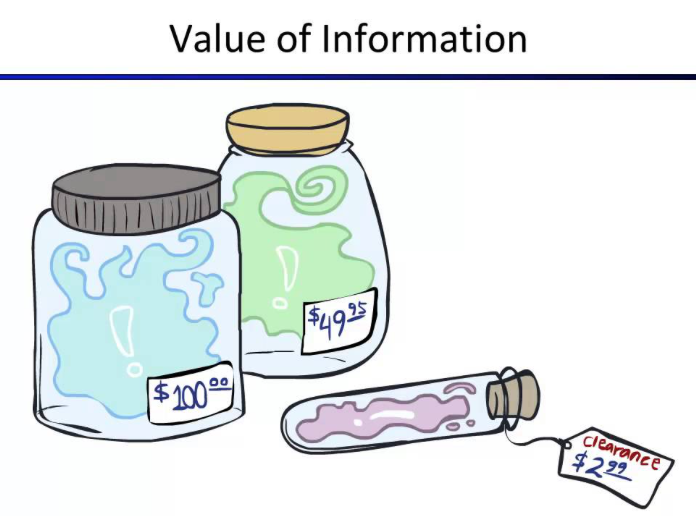
\includegraphics[width=3in]{ValueOfInformation.png} 
      \end{center}

    \lc %{What President hosted Bevo?}
      
    \end{frame}

    %{slide 2}
    \begin{frame}{Topics to Cover}
      \fontsize{10}{10}\selectfont
        \begin{itemize}[<+->]
            \item Value of Information
            \item Bevo: The Movie Example
            \item Expected Value of Perfect Information
            \item Expected Value of Imperfect Information
        \end{itemize}
      
    \end{frame}


    %{slide 3}
    \begin{frame}[fragile]{Value of Information}

        \begin{itemize}[<+->]
            \item Sometimes information can lead to better decisions.
            \item How much is information worth, and if it costs a given amount, should you purchase it?
            \item The expected value of perfect information, or EVPI, is the most you would be willing to pay for perfect information.
        \end{itemize}

     \end{frame}


    %{slide 4}
    \begin{frame}[fragile]{Typical Setup}

      \begin{itemize}[<+->]
        \item In a multistage decision problem, often the first-stage decision is whether to purchase information that will help make a better second stage decision
        \item In this case the information, if obtained, may change the probabilities of later outcomes
        \item In addition, you typically want to learn how much the information is worth
        \item Information usually comes at a price.  You want to know whether the information is worth its price
        \item This leads to an investigation of the value of information
        \end{itemize} 

    \end{frame}



    %{slide 5}
    \begin{frame}[fragile]{Example: Marketing Strategy for Bevo: The Movie}
      \fontsize{10}{10}\selectfont
      UT Productions has to decide on a marketing strategy for it's new movie, Bevo.  Three major strategies are being considered:
      \begin{itemize} [<+->]
        \item (A) Aggressive: Large expenditures on television and print advertising.
        \item (B) Basic: More modest marketing campaign.
        \item (C) Cautious: Minimal marketing campaign.
      \end{itemize} 
      
    \end{frame}



    %{slide 6}
    \begin{frame}[fragile]{Payoffs for Bevo: The Movie}
      \fontsize{10}{10}\selectfont
      The net payoffs depend on the market reaction to the film.

        \begin{center}
          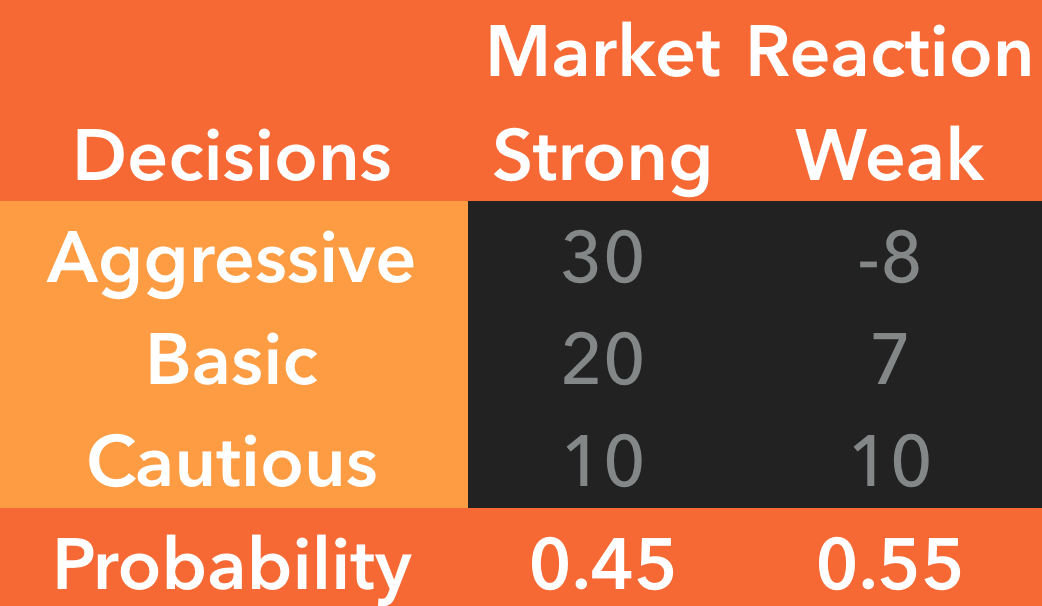
\includegraphics[width=2.5in]{BevoPayoffs} 
        \end{center}
  
    \end{frame}


    %{slide 7}
    \begin{frame}[fragile]{Decision Tree for Bevo: The Movie}

        \begin{center}
          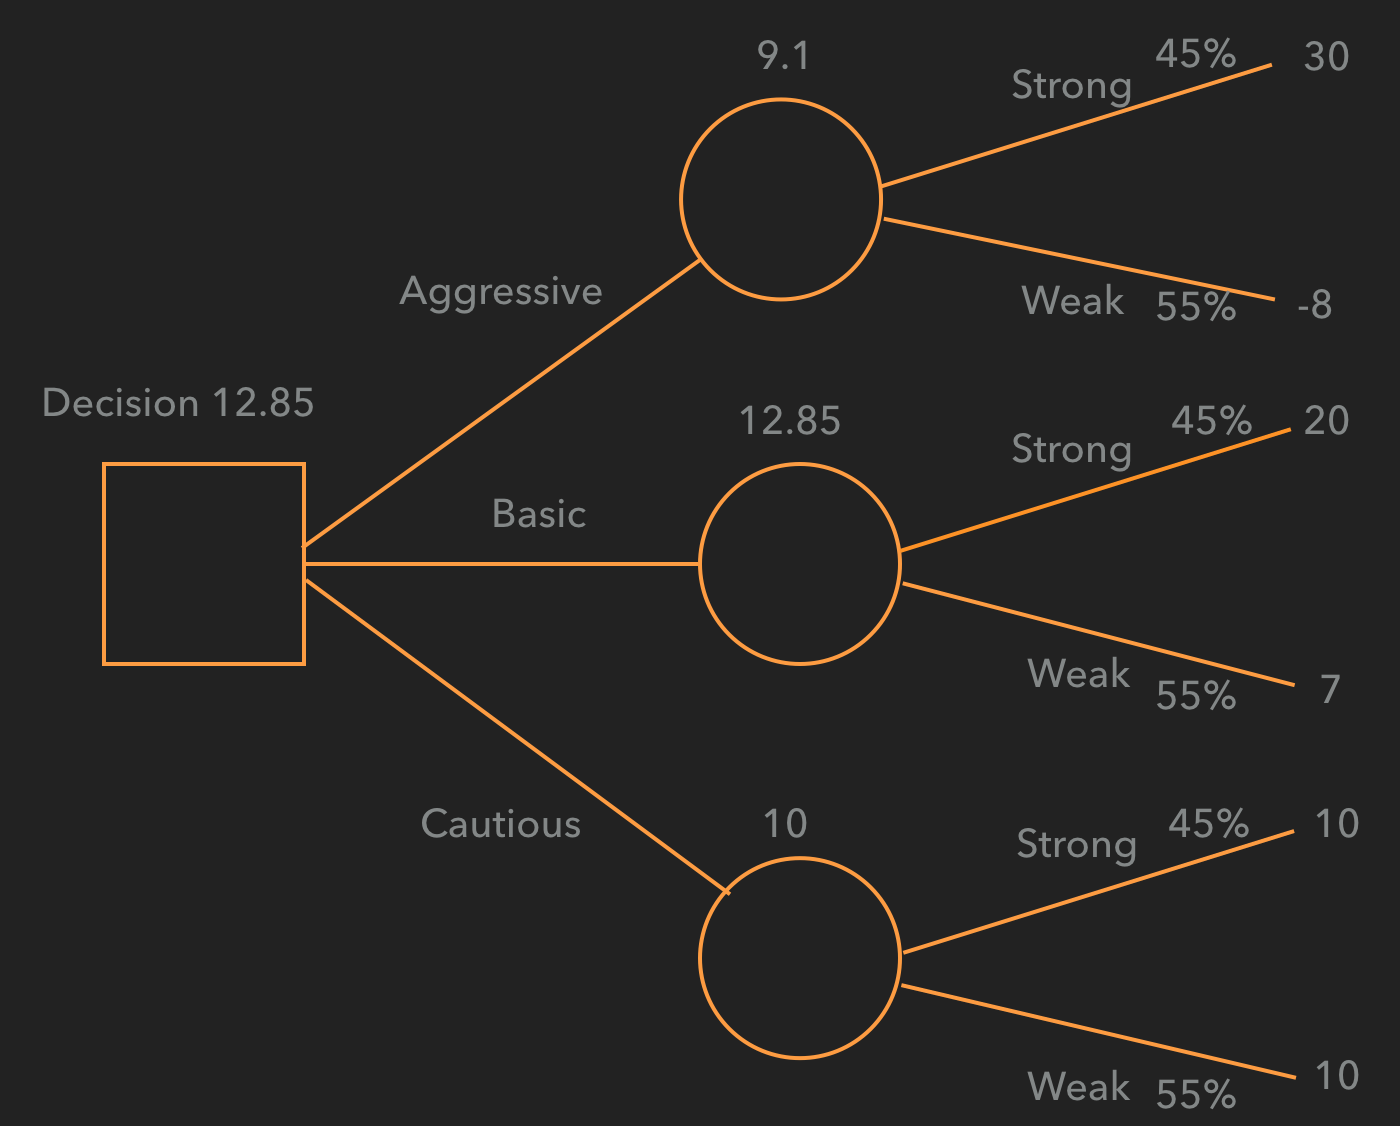
\includegraphics[width=3.5in]{BevoDecisionTree} 
        \end{center}

      \lc %{What would the EV be if there were only two possible strategies, Aggressive and Cautious?}
    \end{frame}


    %{slide 8}
    \begin{frame}[fragile]{Expected Value of Perfect Information (EVPI)}
        \fontsize{10}{10}\selectfont
        How valuable would it be to know what was going to happen?
          \begin{itemize} [<+->]
            \item If a clairvoyant were available to tell you what is going to happen, how much would you pay her?
            \item Assume that you don't know what the clairvoyant will say and you have to pay her before she reveals the answer
          \end{itemize}  
          \pause
          EVPI is: 
             EV with perfect information - EV with no information
    \end{frame}


    %{slide 9}
    \begin{frame}[fragile]{Finding EVPI With a Payoff Table}
      \fontsize{10}{10}\selectfont
      The payoffs depend on the market reaction to the film:
        \begin{center}
        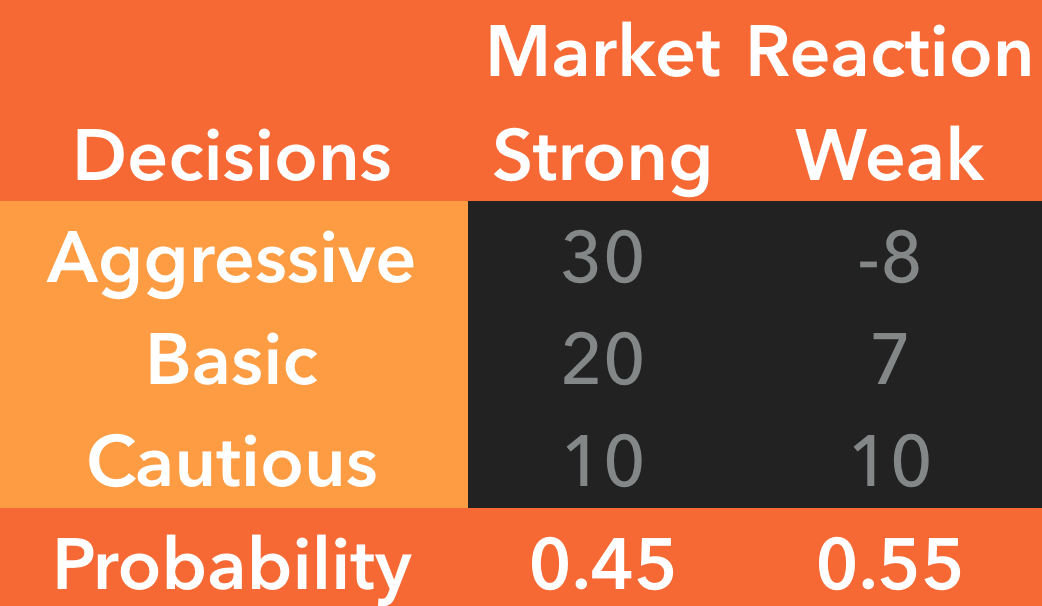
\includegraphics[width=2.5in]{BevoPayoffs} 
        \end{center}
        \begin{itemize} [<+->]
          \item With no information, the Basic strategy is best: EV = 0.45(20) + 0.55(7) = 12.85
          \item With perfect info, select the Agressive strategy for a Strong reaction and the Cautious strategy for a Weak reaction: EV = 0.45(30) + 0.55(10) = 19
          \item EVPI = 19 - 12.85 = 6.15
        \end{itemize}        
    \end{frame}     



   %{slide 10}
    \begin{frame}[fragile]{Finding EVPI With a Decision Tree}
       \fontsize{10}{10}\selectfont   
          \begin{itemize} [<+->]
            \item Step 1: Set up tree without perfect information and calculate EV by rolling back
            \item Step 2: Rearrange the tree the reflect the receipt of the information and calculate the new EV
            \item Step 3: Compare the EV's with and without the information
          \end{itemize}          

    \end{frame}


    %{slide 11}
    \begin{frame}[fragile]{Finding EVPI With a Decision Tree}
      \fontsize{10}{10}\selectfont

        \begin{center}
        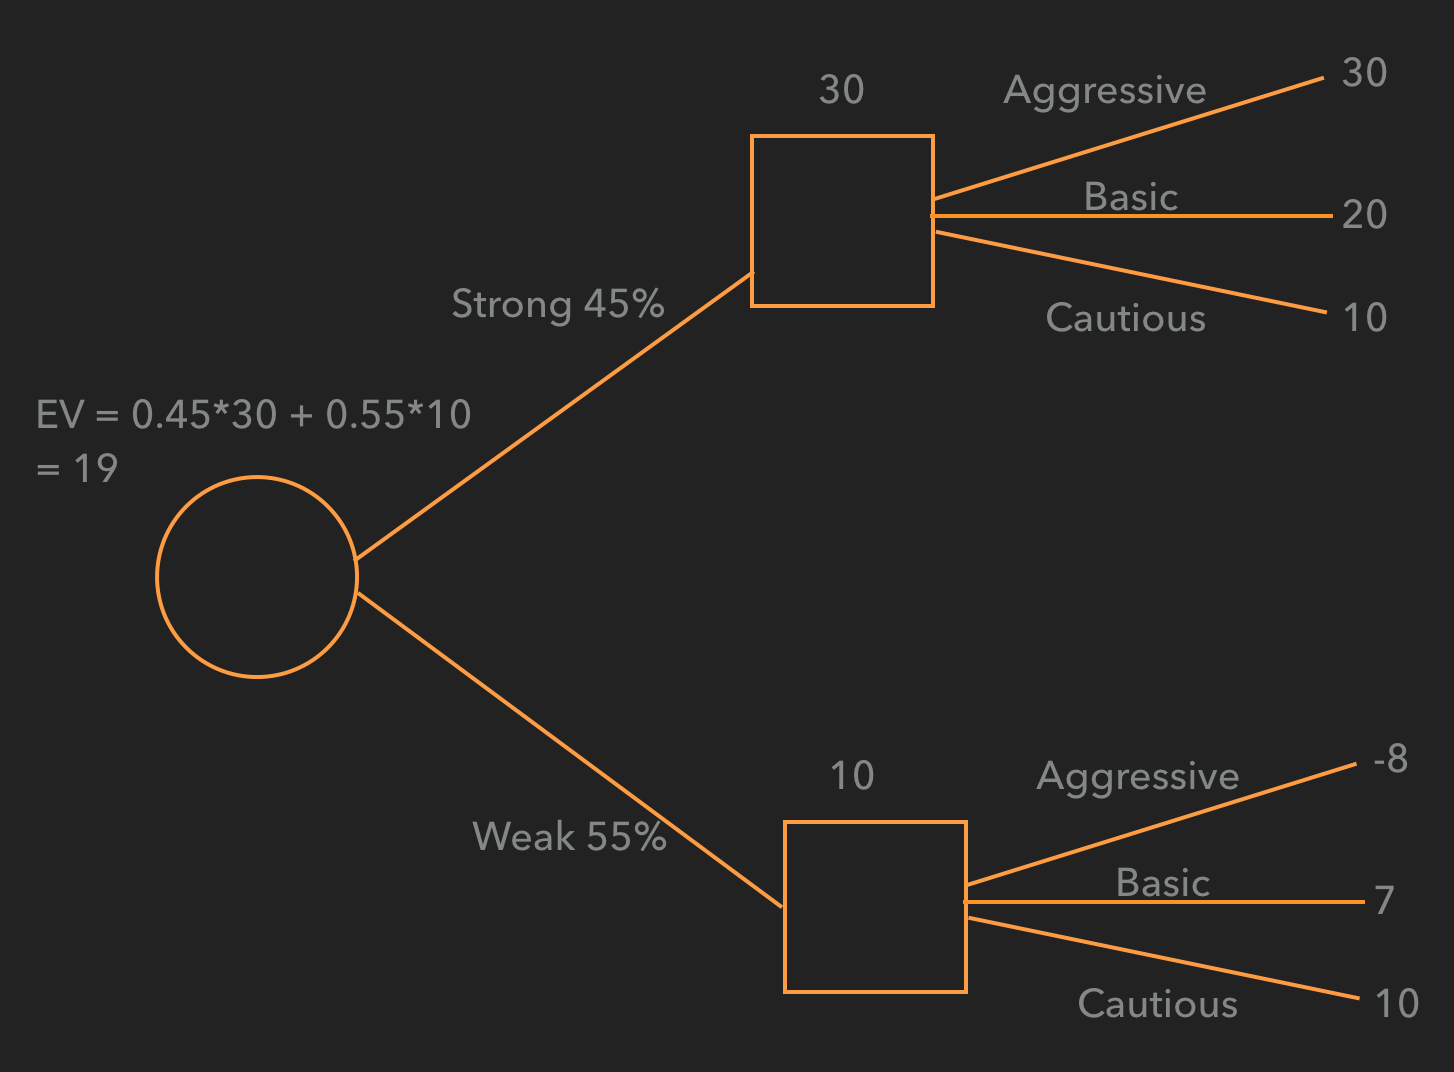
\includegraphics[width=3.5in]{BevoPerfectInfo} 
        \end{center}
    
    \lc %{What would the value of the information be if the payoff was 50 instead of 30 for an Aggressive strategy}
    \end{frame}  


    %{slide 11}
    \begin{frame}[fragile]{What About Imperfect Information?}
      Suppose that Myra the movie critic has a good record of picking winners
      \begin{itemize} [<+->]
        \item In the past, Myra predicted Strong for 70 percent of movies where the audience reaction was Strong and Weak for 30 percent of them.
        \item Similarly, she predicted Weak for 80 percent of movies where the audience reaction was Weak and predicted Strong for 20 percent of them.
        \item Also, remember that the probability of a Strong reaction is 45 percent and of a Weak reaction is 55 percent
      \end{itemize}

      \pause
      What to do now???

      \lc %{How much do you think Myra's information is worth?}
    \end{frame}


    %{slide 12}
    \begin{frame}[fragile]{Reverse the Tree!}

      \begin{center}
        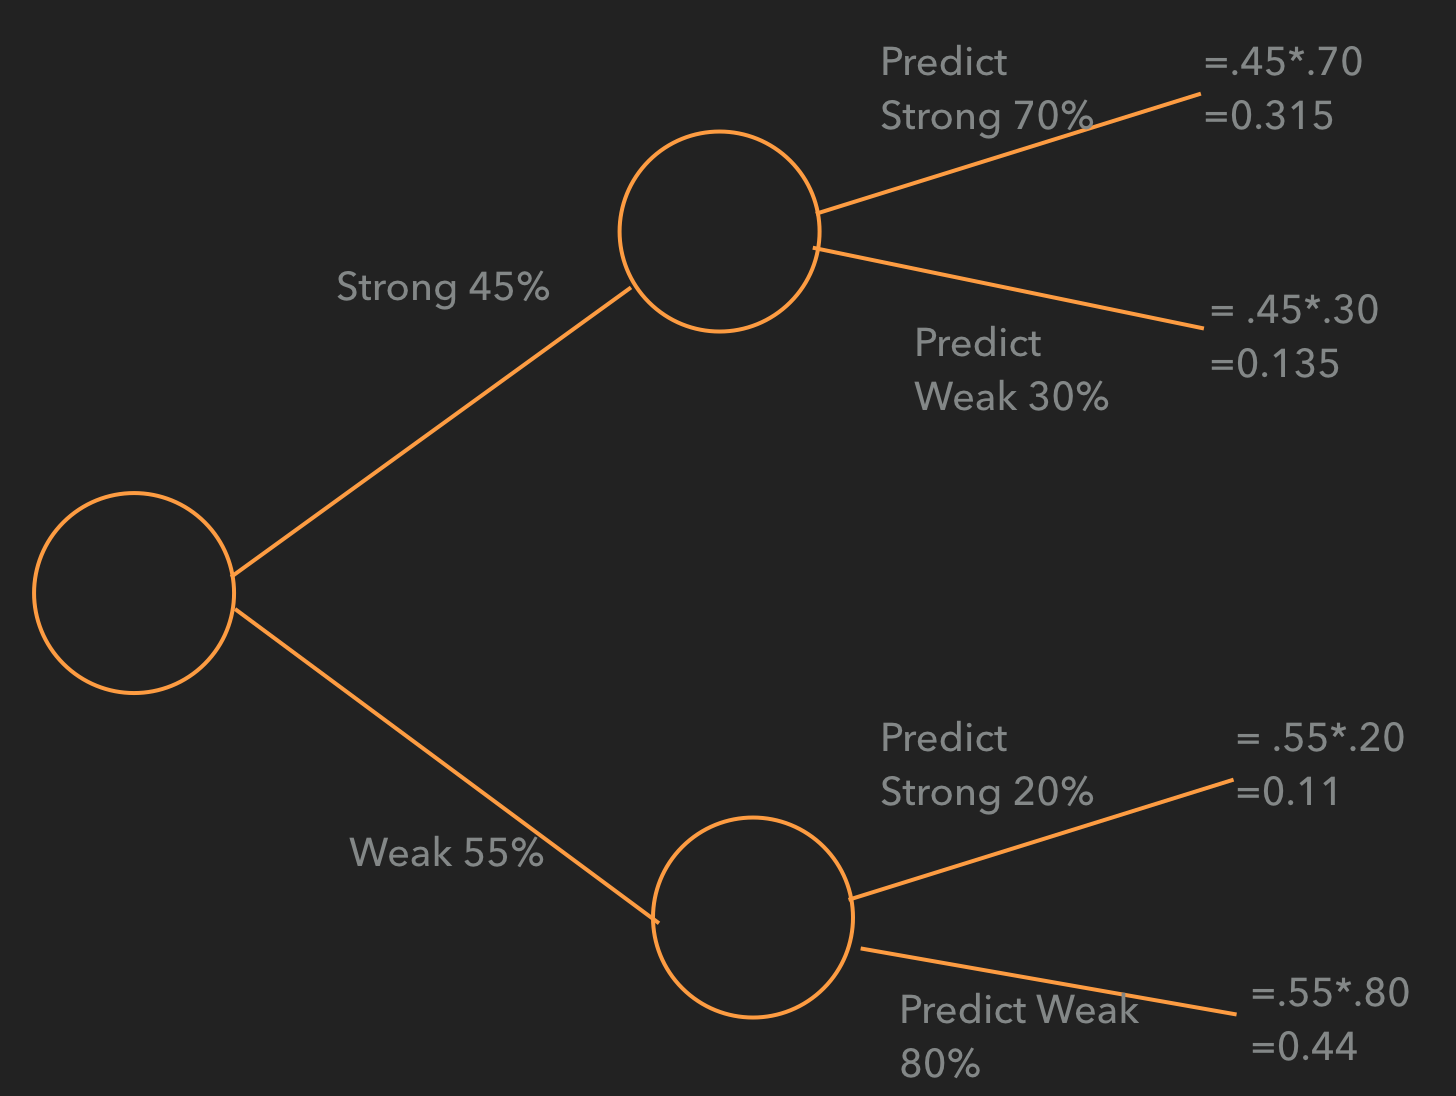
\includegraphics[width=3.5in]{BeforeFlip} \\
      \end{center}

    \end{frame}


    %{slide 13}
    \begin{frame}[fragile]{Reverse the Tree!}

      \begin{center}
        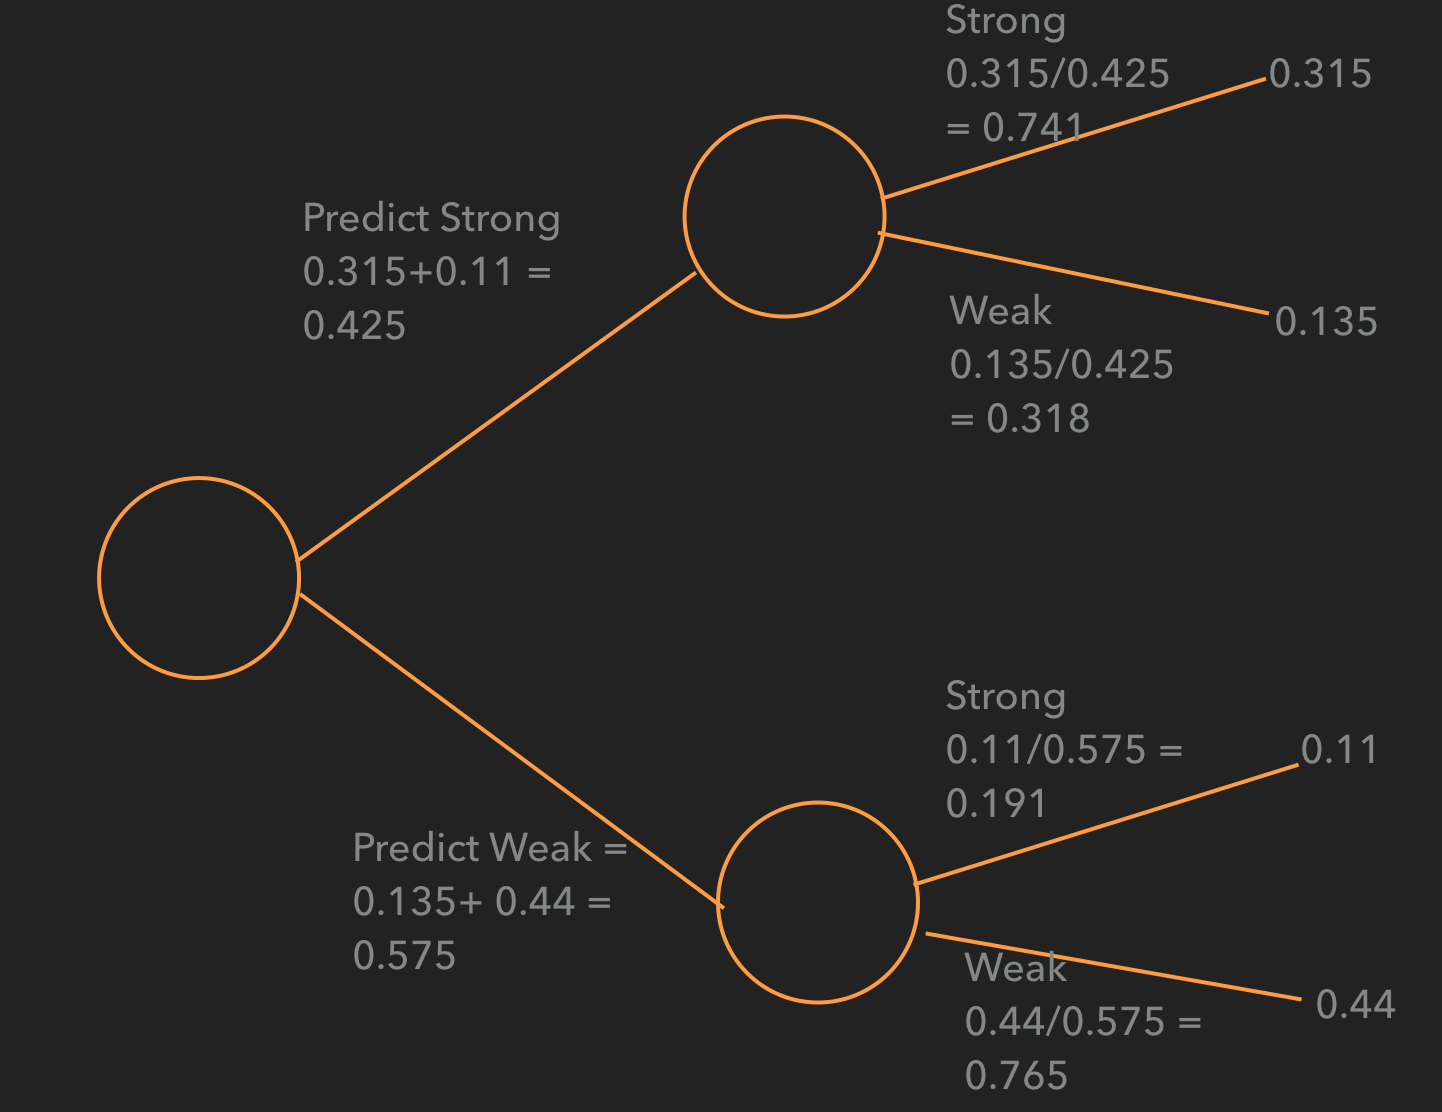
\includegraphics[width=3.5in]{AfterFlip} \\
      \end{center}

    \end{frame}


    %{slide 14}
    \begin{frame}[fragile]{Tree With Imperfect Information}
       
      \begin{center}
        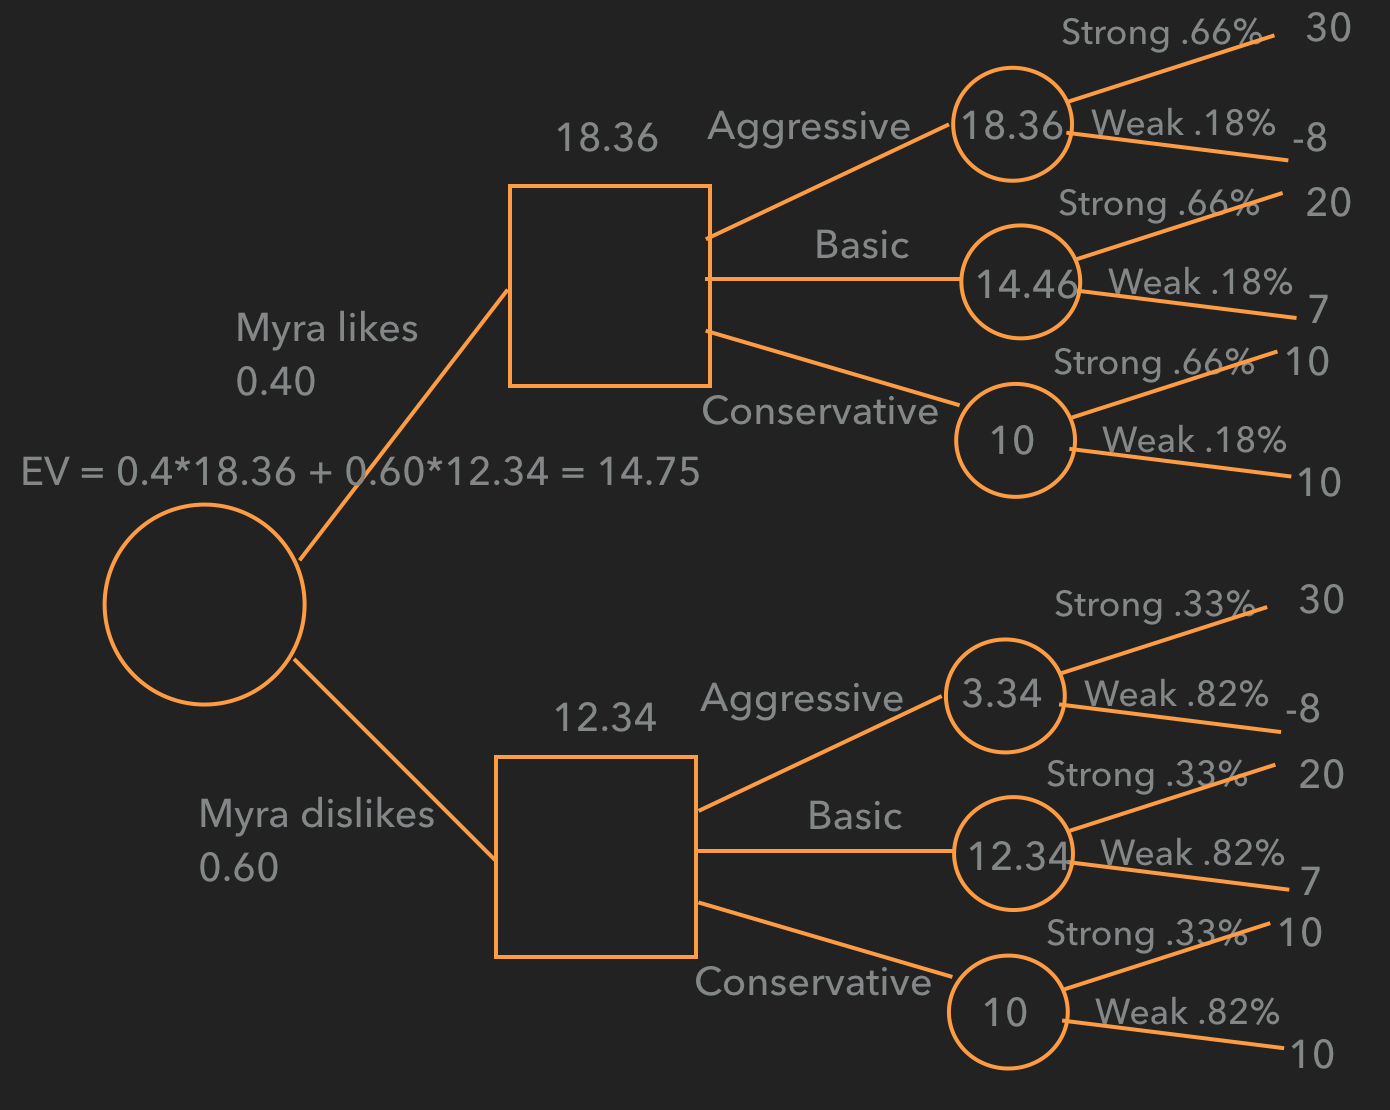
\includegraphics[width=3.5in]{BevoImperfect} \\
      \end{center}

    \end{frame}


    %{slide 15}
    \begin{frame}[fragile]{Myra's Information is Is Worth Paying For}
       It changes the decision and adds 13.65 - 12.85 = 0.80 in value 
      \begin{center}
        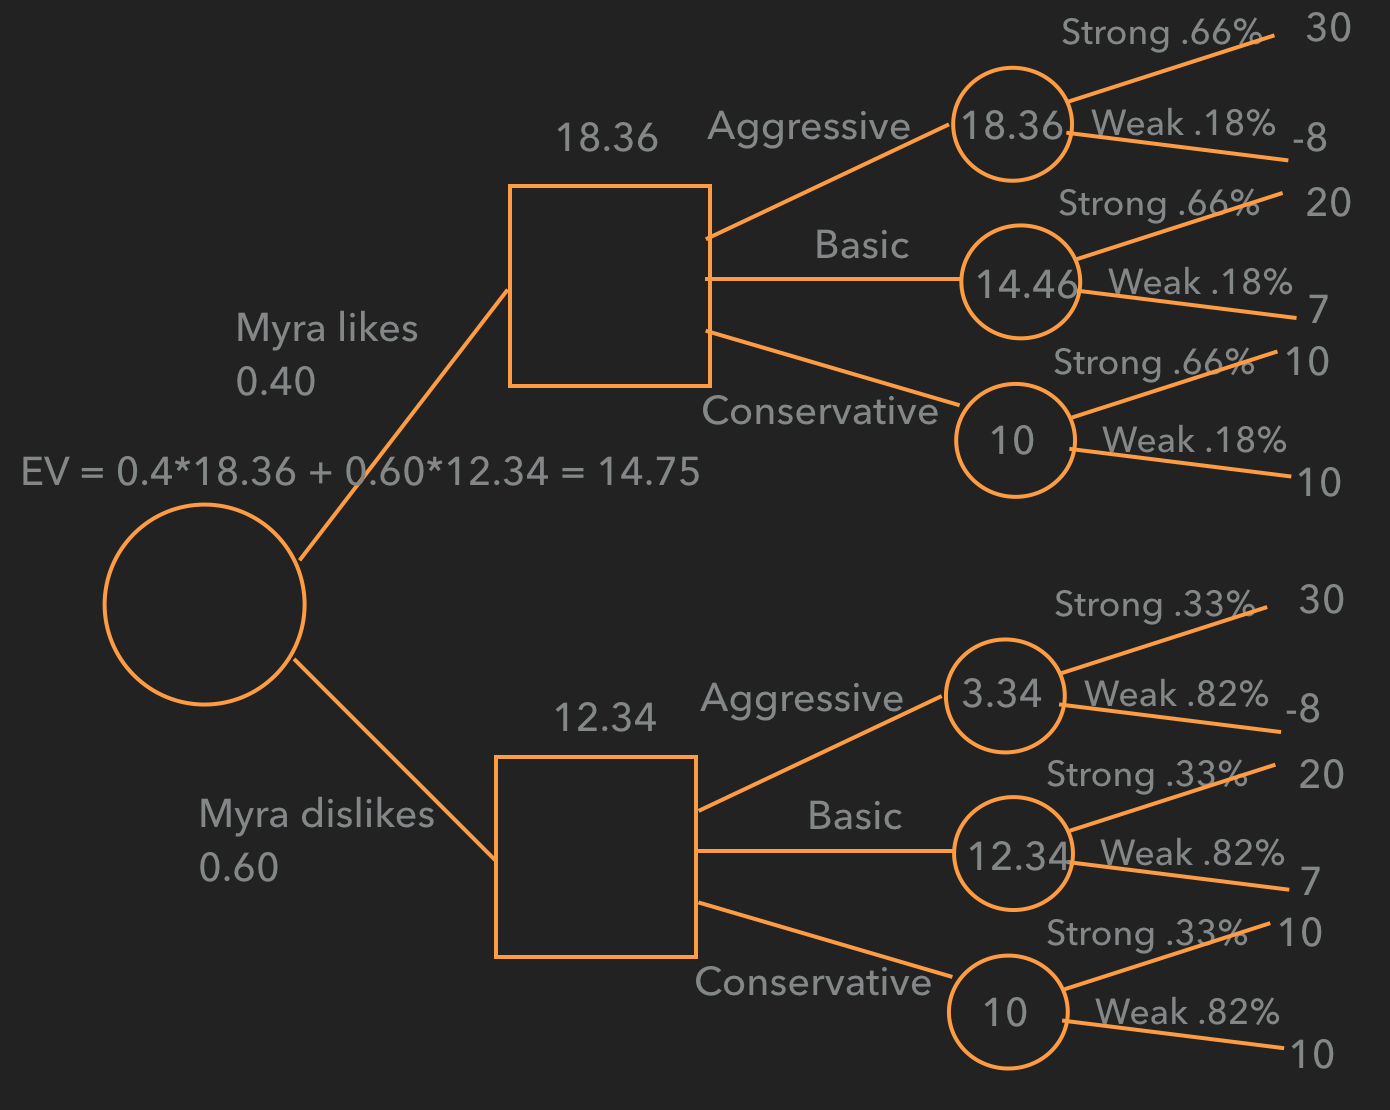
\includegraphics[width=3.5in]{BevoImperfect} \\
      \end{center}

    \end{frame}


    %{slide 16}
    \begin{frame}[fragile]{Things to Remember About Information Value}
       \fontsize{10}{10}\selectfont   
          \begin{itemize} [<+->]
            \item Perfect information is more valuable that any imperfect information
            \item Information cannot have negative value
            \item Information has non-zero value if and only if it changes some decision
            \item Sometimes there is more than one correct way to draw a decision tree for a decision
          \end{itemize}   
    \end{frame}

  \end{darkframes}
\end{document}
